\documentclass[10pt]{article}
\usepackage{fullpage,enumitem,amsmath,amssymb,graphicx,listings,tikz,bbm,xcolor}
\setlength{\parindent}{0pt}

\begin{document}

\begin{center}
{\Large \textbf{Theory Problems: Batch 1}}

\begin{tabular}{rl}
\\
Course: & Coursera Algorithms Specialization \\
Name: & Bryan Yaggi
\end{tabular}
\end{center}

\section*{\normalsize Problem 1}

You are given as input an unsorted array of $n$ distinct numbers, where $n$ is a power of 2. Give an algorithm that identifies the second-largest number in the array, and that uses at most $n + \log⁡_2 n - 2$ comparisons.
\bigskip

The algorithm consists of 2 main steps.

\begin{enumerate}
	\item Compare pairs of consecutive elements until finding the largest. For each element, store a list containing elements with which it was compared.
	\item Find the largest element in the list of elements compared with the largest element. The result is the second largest element.
\end{enumerate}

Step 1 requires $n - 1$ comparisons. Step 2 requires $\log_2 n - 1$ comparisons. The total is $n + \log_2 n - 2$ comparisons.
\smallskip

Example: Given $[4, 8, 3, 7, 2, 6, 1, 5]$.

\begin{center}
  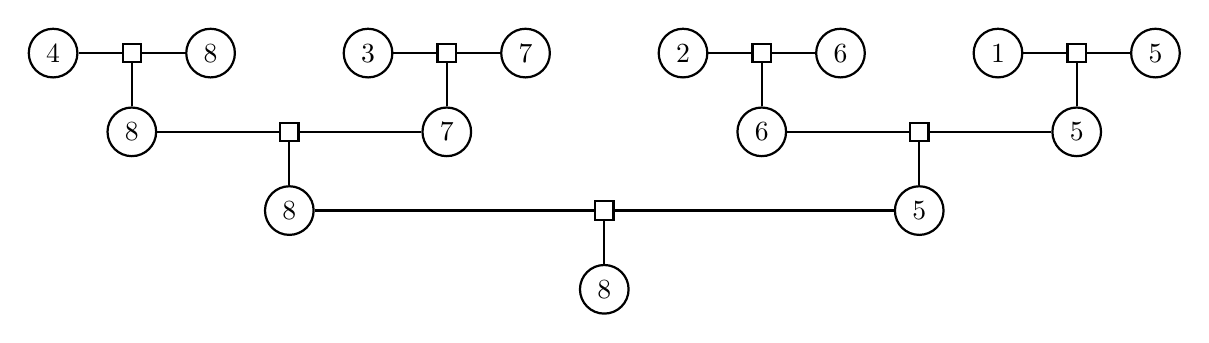
\begin{tikzpicture}
		\begin{scope}[every node/.style={circle,thick,draw}]
    		\node (C11) at (0,0) {$4$};
    		\node (C12) at (2,0) {$8$};
    		\node (C13) at (4,0) {$3$};
    		\node (C14) at (6,0) {$7$};
    		\node (C15) at (8,0) {$2$};
    		\node (C16) at (10,0) {$6$};
    		\node (C17) at (12,0) {$1$};
    		\node (C18) at (14,0) {$5$};
    		\node (C21) at (1,-1) {$8$};
    		\node (C22) at (5,-1) {$7$};
    		\node (C23) at (9,-1) {$6$};
    		\node (C24) at (13,-1) {$5$};
    		\node (C31) at (3,-2) {$8$};
    		\node (C32) at (11,-2) {$5$};
    		\node (C41) at (7,-3) {$8$};
		\end{scope}
		\begin{scope}[every node/.style={rectangle,thick,draw}]
    		\node (f1) at (1,0) {};
    		\node (f2) at (5,0) {};
    		\node (f3) at (9,0) {};
    		\node (f4) at (13,0) {};
    		\node (f5) at (3,-1) {};
    		\node (f6) at (11,-1) {};
    		\node (f7) at (7,-2) {};
		\end{scope}
		\begin{scope}[every edge/.style={draw=black,thick}]
			\path [-] (C11) edge node {} (f1);
			\path [-] (C12) edge node {} (f1);
			\path [-] (C13) edge node {} (f2);
			\path [-] (C14) edge node {} (f2);
			\path [-] (C15) edge node {} (f3);
			\path [-] (C16) edge node {} (f3);
			\path [-] (C17) edge node {} (f4);
			\path [-] (C18) edge node {} (f4);
			\path [-] (C21) edge node {} (f1);
			\path [-] (C22) edge node {} (f2);
			\path [-] (C23) edge node {} (f3);
			\path [-] (C24) edge node {} (f4);
			\path [-] (C21) edge node {} (f5);
			\path [-] (C22) edge node {} (f5);
			\path [-] (C23) edge node {} (f6);
			\path [-] (C24) edge node {} (f6);
			\path [-] (C31) edge node {} (f5);
			\path [-] (C32) edge node {} (f6);
			\path [-] (C31) edge node {} (f7);
			\path [-] (C32) edge node {} (f7);
			\path [-] (C41) edge node {} (f7);
		\end{scope}
	\end{tikzpicture}
\end{center}

The second largest element is $7$, which is the largest of $[4, 7, 5]$.

\section*{\normalsize Problem 2}

You are a given a \textit{unimodal} array of $n$ distinct elements, meaning that its entries are in increasing order up until its maximum element, after which its elements are in decreasing order. Give an algorithm to compute the maximum element that runs in $O(\log n)$ time.
\bigskip

Treat the array as a binary tree with the root as the middle element. Recursively, the middle elements of the resulting subarrays are the next nodes in the tree. Use binary search checking the value of the middle node with its neighbors until the peak is found.

\section*{\normalsize Problem 3}

You are given a sorted (from smallest to largest) array $A$ of $n$ distinct integers which can be positive, negative, or zero. You want to decide whether or not there is an index $i$ such that $A[i] = i$. Design the fastest algorithm that you can for solving this problem.
\bigskip

Again, treat the array as a binary tree. Use binary search to find the solution. If $A[i] < i$, go right. If $A[i] > i$, go left. The algorithm will run in $O(\log n)$ time.

\section*{\normalsize Problem 4}

You are given an $n$ by $n$ grid of distinct numbers. A number is a local minimum if it is smaller than all of its neighbors. (A neighbor of a number is one immediately above, below, to the left, or the right. Most numbers have four neighbors; numbers on the side have three; the four corners have two.) Use the divide-and-conquer algorithm design paradigm to compute a local minimum with only $O(n)$ comparisons between pairs of numbers. (\textbf{Note}: since there are $n^2$ numbers in the input, you cannot afford to look at all of them. \textbf{Hint}: Think about what types of recurrences would give you the desired upper bound.)
\bigskip

The algorithm consists of 2 recursive steps. We will find a local minimum, but not necessarily the global minimum.

\begin{enumerate}
	\item Take the middle row, middle column, and border elements of the 2D array. Find the minimum element of this set.
	\item Find the minimum of the element found in Step 1 and its neighbors. If the minimum is not the element found in Step 1, select the quadrant in which the minimum element lies and recurse.
\end{enumerate}

Step 1 requires $6n - 9$ comparisons. Step 2 requires 2 comparisons. The total is $6n - 7$ for each recursion. Using the master method, $T(n) = a T(\frac{n}{b}) + O(n^d) = T(\frac{n}{2}) + O(n) \therefore O(n)$
\smallskip

Example:

\begin{center}
  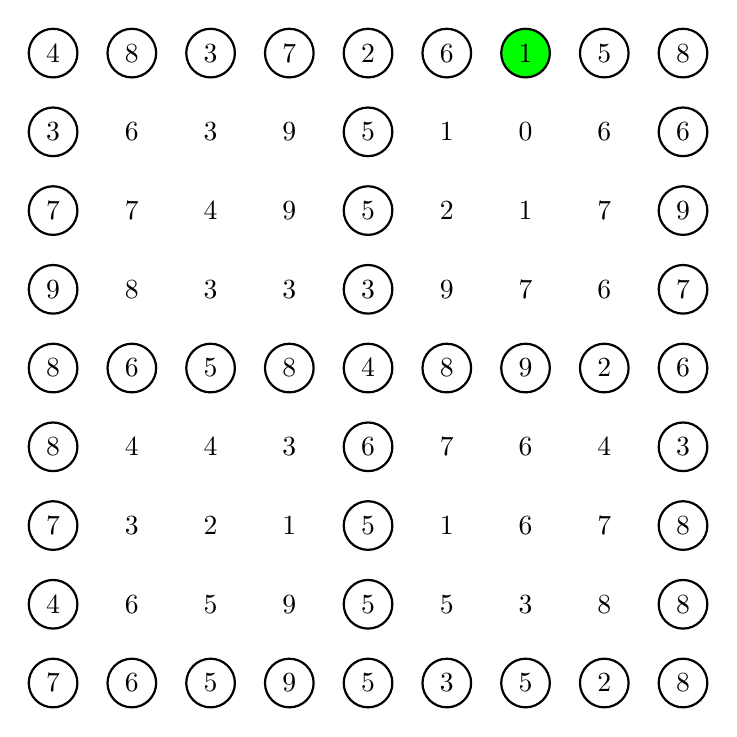
\begin{tikzpicture}
		\begin{scope}[every node/.style={circle,thick,draw}]
    		\node (C11) at (0,0) {$4$};
    		\node (C12) at (1,0) {$8$};
    		\node (C13) at (2,0) {$3$};
    		\node (C14) at (3,0) {$7$};
    		\node (C15) at (4,0) {$2$};
    		\node (C16) at (5,0) {$6$};
    		\node (C18) at (7,0) {$5$};
    		\node (C19) at (8,0) {$8$};
    		\node (C21) at (0,-1) {$3$};
    		\node (C25) at (4,-1) {$5$};
    		\node (C29) at (8,-1) {$6$};
    		\node (C31) at (0,-2) {$7$};
    		\node (C35) at (4,-2) {$5$};
    		\node (C39) at (8,-2) {$9$};
    		\node (C41) at (0,-3) {$9$};
    		\node (C45) at (4,-3) {$3$};
    		\node (C49) at (8,-3) {$7$};
    		\node (C51) at (0,-4) {$8$};
    		\node (C52) at (1,-4) {$6$};
    		\node (C53) at (2,-4) {$5$};
    		\node (C54) at (3,-4) {$8$};
    		\node (C55) at (4,-4) {$4$};
    		\node (C56) at (5,-4) {$8$};
    		\node (C57) at (6,-4) {$9$};
    		\node (C58) at (7,-4) {$2$};
    		\node (C59) at (8,-4) {$6$};
    		\node (C61) at (0,-5) {$8$};
    		\node (C65) at (4,-5) {$6$};
    		\node (C69) at (8,-5) {$3$};
    		\node (C71) at (0,-6) {$7$};
    		\node (C75) at (4,-6) {$5$};
    		\node (C79) at (8,-6) {$8$};
    		\node (C81) at (0,-7) {$4$};
    		\node (C85) at (4,-7) {$5$};
    		\node (C89) at (8,-7) {$8$};
    		\node (C91) at (0,-8) {$7$};
    		\node (C92) at (1,-8) {$6$};
    		\node (C93) at (2,-8) {$5$};
    		\node (C94) at (3,-8) {$9$};
    		\node (C95) at (4,-8) {$5$};
    		\node (C96) at (5,-8) {$3$};
    		\node (C97) at (6,-8) {$5$};
    		\node (C98) at (7,-8) {$2$};
    		\node (C99) at (8,-8) {$8$};
		\end{scope}
		\begin{scope}[]
    		\node (C22) at (1,-1) {$6$};
    		\node (C23) at (2,-1) {$3$};
    		\node (C24) at (3,-1) {$9$};
    		\node (C26) at (5,-1) {$1$};
    		\node (C27) at (6,-1) {$0$};
    		\node (C28) at (7,-1) {$6$};
    		\node (C32) at (1,-2) {$7$};
    		\node (C33) at (2,-2) {$4$};
    		\node (C34) at (3,-2) {$9$};
    		\node (C36) at (5,-2) {$2$};
    		\node (C37) at (6,-2) {$1$};
    		\node (C38) at (7,-2) {$7$};
    		\node (C42) at (1,-3) {$8$};
    		\node (C43) at (2,-3) {$3$};
    		\node (C44) at (3,-3) {$3$};
    		\node (C46) at (5,-3) {$9$};
    		\node (C47) at (6,-3) {$7$};
    		\node (C48) at (7,-3) {$6$};
    		\node (C62) at (1,-5) {$4$};
    		\node (C63) at (2,-5) {$4$};
    		\node (C64) at (3,-5) {$3$};
    		\node (C66) at (5,-5) {$7$};
    		\node (C67) at (6,-5) {$6$};
    		\node (C68) at (7,-5) {$4$};
    		\node (C72) at (1,-6) {$3$};
    		\node (C73) at (2,-6) {$2$};
    		\node (C74) at (3,-6) {$1$};
    		\node (C76) at (5,-6) {$1$};
    		\node (C77) at (6,-6) {$6$};
    		\node (C78) at (7,-6) {$7$};
    		\node (C82) at (1,-7) {$6$};
    		\node (C83) at (2,-7) {$5$};
    		\node (C84) at (3,-7) {$9$};
    		\node (C86) at (5,-7) {$5$};
    		\node (C87) at (6,-7) {$3$};
    		\node (C88) at (7,-7) {$8$};
		\end{scope}
		\begin{scope}[every node/.style={circle,thick,draw,fill=green}]
    		\node (C17) at (6,0) {$1$};
		\end{scope}
	\end{tikzpicture}
\end{center}

\begin{center}
  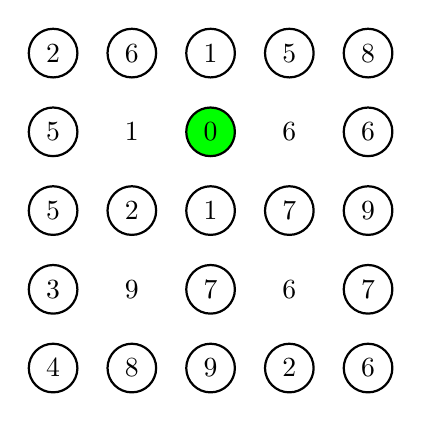
\begin{tikzpicture}
		\begin{scope}[every node/.style={circle,thick,draw}]
    		\node (C15) at (4,0) {$2$};
    		\node (C16) at (5,0) {$6$};
    		\node (C17) at (6,0) {$1$};
    		\node (C18) at (7,0) {$5$};
    		\node (C19) at (8,0) {$8$};
    		\node (C25) at (4,-1) {$5$};
    		\node (C29) at (8,-1) {$6$};
    		\node (C35) at (4,-2) {$5$};
    		\node (C36) at (5,-2) {$2$};
    		\node (C37) at (6,-2) {$1$};
    		\node (C38) at (7,-2) {$7$};
    		\node (C39) at (8,-2) {$9$};
    		\node (C45) at (4,-3) {$3$};
    		\node (C47) at (6,-3) {$7$};
    		\node (C49) at (8,-3) {$7$};
    		\node (C55) at (4,-4) {$4$};
    		\node (C56) at (5,-4) {$8$};
    		\node (C57) at (6,-4) {$9$};
    		\node (C58) at (7,-4) {$2$};
    		\node (C59) at (8,-4) {$6$};
		\end{scope}
		\begin{scope}[]
    		\node (C26) at (5,-1) {$1$};
    		\node (C28) at (7,-1) {$6$};
    		\node (C46) at (5,-3) {$9$};
    		\node (C48) at (7,-3) {$6$};
		\end{scope}
		\begin{scope}[every node/.style={circle,thick,draw,fill=green}]
    		\node (C27) at (6,-1) {$0$};
		\end{scope}
	\end{tikzpicture}
\end{center}

\end{document}
